\documentclass[twocolumn, 8pt]{extarticle}

% Uncomment to squeeze everything onto one side
%\usepackage{pgfpages}
%\pgfpagesuselayout{2 on 1}[letterpaper, landscape]

\usepackage[letterpaper,margin=0.25in]{geometry}
\input{ncommon}
\everymath{}
\usepackage{titlesec}
\usepackage{enumitem}
\usepackage{multicol}

% Options: [subtle], [moderate], or [extreme]
\usepackage[extreme, mathspacing=normal]{savetrees}

\titleformat{\section}
  {\normalfont\fontsize{12}{14}\bfseries}{\thesection}{1em}{}
\titlespacing\section{0pt}{5pt plus 2pt minus 2pt}{2pt plus 1pt minus 1pt}
\titlespacing\subsection{0pt}{5pt plus 2pt minus 2pt}{2pt plus 1pt minus 1pt}
\titlespacing\subsubsection{0pt}{5pt plus 2pt minus 2pt}{2pt plus 1pt minus 1pt}
%\renewcommand{\arraystretch}{1.5}
\setlist{nosep}
\setlength{\abovedisplayskip}{3pt}
\setlength{\belowdisplayskip}{3pt}
\setlength{\abovedisplayshortskip}{0pt}
\setlength{\belowdisplayshortskip}{3pt}
\setlength{\parindent}{0pt}
\setlength{\parskip}{2pt}
\raggedbottom
\raggedcolumns

% Normal vdots and ddots leave too much space above
% https://tex.stackexchange.com/questions/207056/wrong-too-much-vertical-space-above-vdots-in-small-matrix
\newcommand{\newvdots}{\vphantom{\int\limits^x}\smash[t]{\vdots}}
\newcommand{\newddots}{\vphantom{\int\limits^x}\smash[t]{\ddots}}

\title{ECE557 Exam Aidsheet}
\author{Tyler Tian}

\begin{document}

\section{Dynamical Systems}

\textbf{LTI System:} \(\dot{\bm x} = \bm A\bm x(t) + \bm B\bm u(t), \bm y(t) = \bm C\bm x(t) + \bm D\bm u(t)\)
where \(\bm A \in \reals^{n \times n}\) (system), \(\bm B \in \reals^{n \times m}\) (input), \(\bm C \in \reals^{p
\times n}\) (output) \(\bm D \in \reals^{p \times m}\) (feedforward)

\textbf{TF to SS:} \(G(s) = N(s)/D(s) \implies D(s)V(s) = U(s), N(s)V(s) = Y(s)\); inverse
Laplace \& let \(x\) be \(v\) and its derivatives, rearrange to get state eqn. from first and measurement eqn. from
second.

\textbf{SS to TF:} \(\bm G(s) = \bm C(s\bm I - \bm A)^{-1}\bm B + \bm D \in \reals^{p \times m}\)

\textbf{Linearization:} Let \(\dot{\bm x} = \bm f(\bm x, \bm u), \bm y = \bm h(\bm x, \bm u)\), let \(\delta\bm x = \bm
x - \bm x^*, \delta\bm u = \bm u - \bm u^*\), the linearized system about \((\bm x^*, \bm u^*)\) is (\(\bm f(\bm x^*,
\bm u^*) = 0\) for eqm. condition):
\begin{align*}
    \delta\dot{\bm x} &= \bm A\delta\bm x + \bm B\delta\bm u + \bm f(\bm x^*, \bm u^*) &&\quad \bm A = \pdiff{\bm f}{\bm x}(\bm x^*, \bm u^*) &\quad \bm B = \pdiff{\bm f}{\bm u}(\bm x^*, \bm u^*) \\
    \bm y &= \bm C\delta\bm x + \bm D\delta\bm u &&\quad \bm C = \pdiff{\bm h}{\bm x}(\bm x^*, \bm u^*) &\quad \bm D = \pdiff{\bm h}{\bm u}(\bm x^*, \bm u^*)
\end{align*}

\textbf{Solutions:} \(\displaystyle \bm x(t) = e^{\bm At}\bm x_0 + \int _0^t e^{\bm A(t - \tau)}\bm B\bm u(\tau)\,\dtau\)

For autonomous (\(\bm u = 0\)) systems, the matrix exponential is the unique soln.

\section{Matrix Exponential \& Diagonalization}

\textbf{Matrix Exponential:} \(e^{\bm A} = \sum _{k = 0}^\infty \frac{1}{k!}\bm A^k\) has the following properties:
\begin{enumerate}
    \item For all invertible \(\bm P \in \reals^{n \times n}\), \(e^{\bm P\bm A\bm P^{-1}} = \bm Pe^{\bm A}\bm P^{-1}\).
    \item \(e^{\bm A + \bm B} = e^{\bm A}e^{\bm B} = e^{\bm B}e^{\bm A}\) if \(\bm A\bm B = \bm B\bm A\).
    \item Matrix exponential is always invertible: \((e^{\bm A})^{-1} = e^{-\bm A}\).
    \item \(\forall t \in \reals, \diff{}{t}e^{\bm At} = \bm Ae^{\bm At} = e^{\bm At}\bm A\).
\end{enumerate}

\textbf{From Laplace Transform:} \(\bm e^{\bm At} = \ilaplace{(s\bm I - \bm A)^{-1}}\)

\textbf{Diagonalization:} \(\bm P^{-1}\bm A\bm P = \bm\Lambda\) where \(\bm P\) has e'vects, \(\bm\Lambda\) is diagonal
with e'vals. Possible if and only if \(\bm A\) has \(n\) lin. indep. e'vects, then \(e^{\bm A} = \bm Pe^{\bm\Lambda}\bm P^{-1}\).

If \(\bm A\) has \(n\) distinct eigenvalues or if \(\bm A\) is symmetric, it's always diagonalizable.

\textbf{Complex Eigenvalues:} Conjugate pairs; can find real \(\tilde{\bm P}\tilde{\bm\Lambda}\tilde{\bm P}^{-1} = \bm A\):
\begin{gather*}
    \tilde{\bm P} = \rvec{\bm v_r}{\Re(\bm v_c)}{\Im(\bm v_c)} \qquad
    \tilde{\bm\Lambda} = \matthree{\lambda _r}{0}{0}{0}{\Re(\lambda _c)}{\Im(\lambda _c)}{0}{-\Im(\lambda _c)}{\Re(\lambda _c)} \\
    \exp\left(\mattwo{a}{b}{-b}{a}t\right) = e^{at}\mattwo{\cos(bt)}{\sin(bt)}{-\sin(bt)}{\cos(bt)}
\end{gather*}
For real \(\bm v_r, \lambda _r\), complex \(\bm v_c, \lambda _c\).
Rotation CW if \(b > 0\), CCW if \(b < 0\).

\textbf{Algebraic Multiplicity:} \(m_i\) is the number of times \(\lambda _i\) appears as an eigenvalue of \(\bm A\),
i.e. the power of \(s - \lambda _i\) in \(\det(s\bm I - \bm A)\). \(\sum _i m_i = n\).

\textbf{Geometric Multiplicity:} \(l_i = \dim(\mathcal N(\lambda _i\bm I - \bm A))\), i.e. the number of indep.
e'vects corresponding to \(\lambda _i\). \(l_i \leq m_i\); \(l_i = m_i\) if and only if \(\bm A\) is diagonalizable.

\textbf{Generalized Eigenvector:} \((\lambda\bm I - \bm A)^k\bm v = \bm 0, k \in \naturals\). For each (true) e'vect
\(\bm e = \bm v_1\) for a given \(\lambda\), we can form a chain \((\lambda\bm I - \bm A)\bm v_{k + 1} = -\bm v_k\)
until we have \(m_i\) gen. e'vects in total, and form \(\bm P\) by grouping gen. e'vect chains corresponding to each
true e'vect, then grouping e'vects for each e'val.

\textbf{Jordan Normal Form:} For nondiagonalizable \(\bm A\), \(\bm P^{-1}\bm A\bm P = \bm J\) where
\[\setlength{\arraycolsep}{2pt}
\bm J = \diagthree{\bm J_{\lambda _1}}{\newddots}{\bm J_{\lambda _k}} \quad
\bm J_{\lambda _i} = \diagthree{\bm J_{\lambda _i}^1}{\newddots}{\bm J_{\lambda _i}^{l_i}} \quad
\bm J_{\lambda _i}^j = \begin{bmatrix}\lambda _i & 1 & & \\[-1ex] & \lambda _i & \newddots & \\[-1ex] & & \newddots & 1 \\ & & & \lambda _i \end{bmatrix}\]
Each \(\bm J_{\lambda _i} \in \complex^{m_i \times m_i}\) corresponds to a distinct e'val. Each \(\bm J_{\lambda _i}^j\)
corresponds to the chain of generalized e'vects for one true e'vect of that eigenspace.
\[\setlength{\arraycolsep}{2pt}
e^{\bm J_{\lambda _i}t} = \diagthree{e^{\bm J_{\lambda _i}^1}}{\newddots}{e^{\bm J_{\lambda _i}^{l_i}}} \quad
e^{\bm J_{\lambda _i}^jt} = e^{\lambda _it}\begin{bmatrix}1 & t & \cdots & \frac{t^{p - 1}}{(p - 1)!} \\ & \newddots & \newddots & \newvdots \\ & & 1 & t \\ & & & 1 \end{bmatrix}\]

\section{System Behaviour \& Stability}

\textbf{Modal Decomposition:} Let \(\bm z(t) = \bm P^{-1}\bm x(t)\), then \(\dot{\bm z} = \bm\Lambda\bm z\), and each
\(z_i(t) = e^{\lambda _it}z_i(0)\). Decompose the solution into modes:
\[\bm x(t) = \bm P\bm z(t) = \sum _{i = 1}^n \bm v_i\bm z_i(t) = \sum _{i = 1}^n \bm v_ie^{\lambda _it}z_i(0) = \sum _{i = 1}^n \bm h_i(t)\]
Geometrically, any initial condition is broken into a linear combination of the modes; in \(z\)-space, the modes become
axis-aligned.

\textbf{Stability:} \(\forall \bm x_0 \in \reals^n, \exists M < \infty \suchthat \norm{\bm x(t)} \leq M,\,\forall t \geq 0\)
(solns. bounded)

\textbf{Asymptotic Stability:} \(\forall \bm x_0 \in \reals^n, \lim _{t \to \infty} x(t) = \bm 0\).
Implies BIBO and input-output stability.

\textbf{BIBO Stability:} For \(\bm x_0 = \bm 0\), \(\bm u(t)\) bounded \(\implies \bm y(t)\) also bounded.
If \(G(s)\) is stable, the system is BIBO stable but not always I/O stable.

\textbf{Input-Output Stability:} For any \(\bm x_0 \in \reals^n\), \(\bm u(t)\) bounded \(\implies \bm y(t)\) also
bounded. Implies BIBO stability.

\textbf{Lyapunov Equation:} If there exists positive definite \(\bm P\) such that \(\bm Q = -\bm A^T\bm P - \bm P\bm A\)
is positive definite, then \(\dot{\bm x} = \bm A\bm x\) is asymptotically stable.

\textbf{Relation to Eigenvalues:} The system is asymptotically stable if and only if \(\Re(\lambda _i) < 0\). If any
\(\Re(\lambda _i) > 0\), it is unstable. For e'vals where \(\Re(\lambda _i) = 0\), the system is stable if and only if
\(m_i = l_i\).

\textbf{System Behaviour According to Eigenvalues:}
\begin{enumerate}
    \item Real nonzero eigenvalues: Stable node if \(\lambda _i < 0\), unstable node if \(\lambda _i > 0\), saddle if mixed signs.
    \item Complex eigenvalues: Stable focus if \(\Re(\lambda _i) < 0\), unstable focus if \(\Re(\lambda _i) > 0\), centre if
          \(\Re(\lambda _i) = 0\).
    \item Zero eigenvalues: Solutions converge or diverge from an equilibrium line.
\end{enumerate}

\vspace{-1em}
\begin{center}
    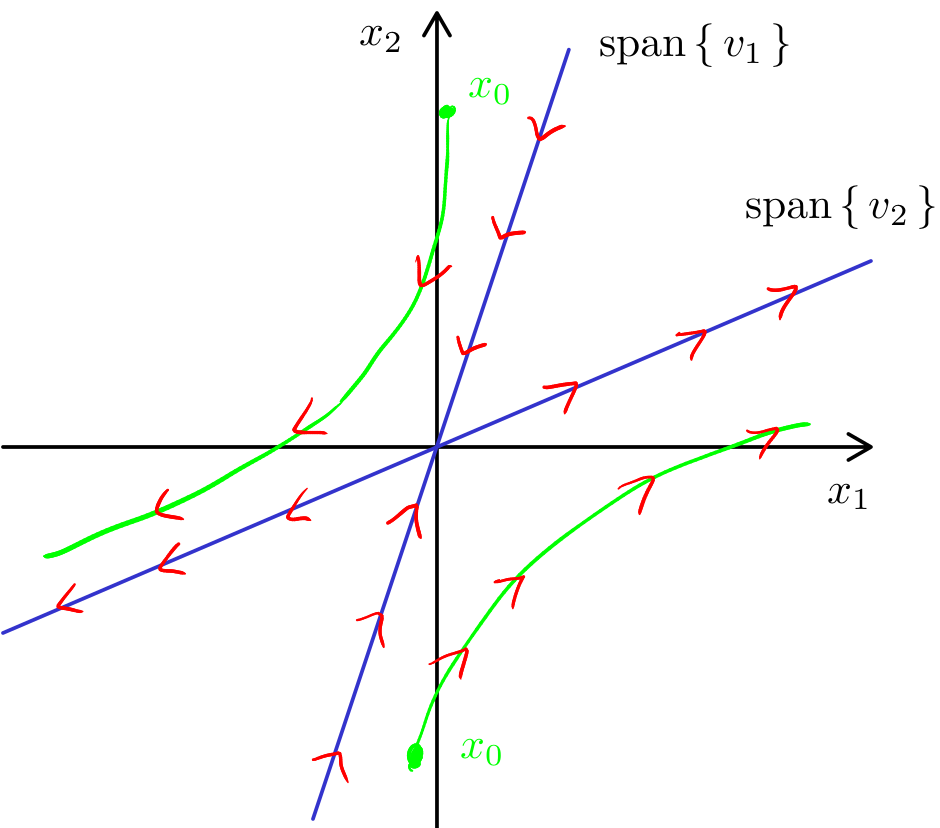
\includegraphics[width=0.3\linewidth]{imgs/eigenvalues_behaviour.png}
    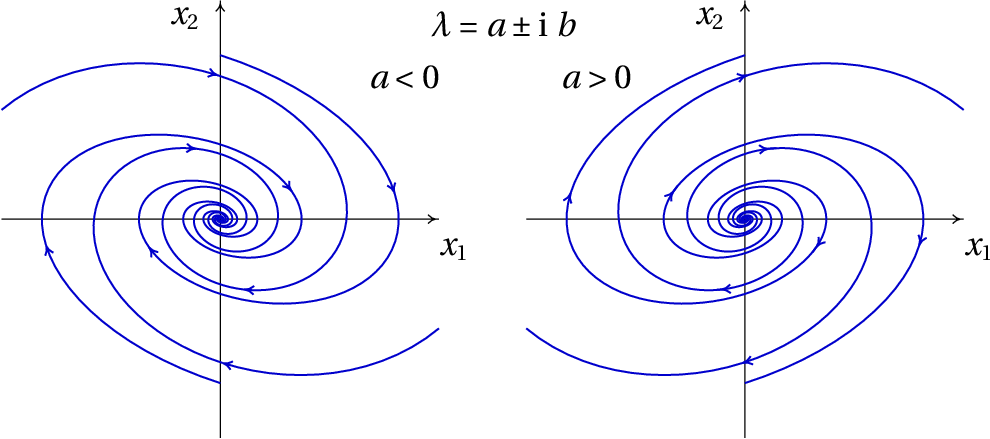
\includegraphics[width=0.6\linewidth]{imgs/focus.png}
\end{center}
\vspace{-1.8em}

\section{Linear Transformations}

\textbf{Vector Space:} Set of vectors, field \(\mathbb F\), operations addition and multiplication, satisfying: 1.
Closure, 2. Addition Commutativity, 3. Associativity, 4. Identity Elements, 5. Additive Inverse, and 6. Distributivity.

\textbf{Span:} \(\Span\set{x_1, \dots, x_m} = \Set{\sum _{i = 1}^m c_ix_i | c_i \in \mathbb F}\)

\textbf{Dimension:} Smallest \(m\) such that \(\mathcal X = \Span\set{x_1, \dots, x_m}\).

\textbf{Linear Independence:} \(\forall c_1, \dots, c_m \in \mathbb F,\, \sum _{i = 1}^m c_ix_i = \theta \iff c_i = 0,\,\forall i\)

\textbf{Basis:} \(\mathcal B = \set{x_1, \dots, x_m} \subseteq \mathcal X\) is a basis if
\(\mathcal X = \Span\mathcal B\) and \(\mathcal B\) is lin. indep.

\textbf{Coordinate Representation:} \(v = \sum _{i = 1}^m c_ix_i\); unique for a given basis.

\textbf{Subspace:} \(\mathcal V \subseteq \mathcal X\) is a subspace if it is closed and contains the zero vector.

\textbf{Direct Sum:} \(\mathcal V \oplus \mathcal W = \set{v + w | v \in \mathcal V, w \in \mathcal W}\); is another subspace.

\textbf{Indep. Comp.:} Subspace where \(\mathcal W \cap \mathcal V = \set{0}\) and \(\mathcal W \oplus
\mathcal V = \mathcal X\).

\textbf{Orthogonal Comp.:} \(\mathcal V^\perp = \set{w \in \mathcal X | \inner{w}{v} = 0,\,\forall v \in \mathcal V}\).
\(\mathcal V^\perp \oplus \mathcal V = \mathcal X\).

\textbf{Injective/One-to-One:} \(\forall x_1, x_2 \in \mathcal X, f(x_1) = f(x_2) \implies x_1 = x_2\)

\textbf{Surjective/Onto:} \(\forall y \in \mathcal Y,\,\exists x \in \mathcal X \suchthat f(x) = y\)

\textbf{Bijective:} Both injective and surjective.

\textbf{Linear Map:} \(\forall x_1, x_2 \in \mathcal X, \lambda \in \mathbb F,\, L(x + \lambda y) = L(x) + \lambda L(y)\)

\textbf{Null Space/Kernel:} \(\mathcal N(L) = \set{\bm x \in \mathcal X | L(\bm x) = \theta}\)

\textbf{Range Space/Image:} \(\mathcal R(L) = \set{\bm y \in \mathcal Y | \exists \bm x \in \mathcal X,\,\bm y = L(\bm x)}\)

\textbf{Rank-Nullity:} \(L: \mathcal X \mapsto \mathcal Y\) satisfies \(\dim(\mathcal R(L)) + \dim(\mathcal N(L)) = \dim(\mathcal X)\).

\textbf{Matrix Representation:} For \(L: \mathcal X \mapsto \mathcal Y\), the \(i\)th column of \(\bm A\) contains the
coordinates of \(L(x^i)\) where \(x^i\) is the \(i\)th basis vector of \(\mathcal X\), under the \(\mathcal Y\) basis.

\(L\) is injective if and only if \(\dim(\mathcal N(\bm A)) = 0\). \(L\) is surjective if and only if \(\rank(\bm A) =
\dim(\mathcal Y)\). \(L\) is bijective if and only if \(\bm A\) is square and invertible.

\textbf{Similarity Transform:} \(L: \reals^n \mapsto \reals^n\) defined as \(L(\bm x) = \bm A\bm x\) expressed in basis
\(\set{\bm v_1, \dots, \bm v_n}\) for \(\reals^n\) is \(\hat{\bm A} = \bm P^{-1}\bm A\bm P\) where \(\bm P = \rvec{\bm
v_1}{\cdots}{\bm v_n}\).

\textbf{Invariant Subspace:} \(\mathcal V\) is \(\bm A\)-invariant (\(\bm A\mathcal V \subseteq \mathcal V\)) if
\(\forall\bm x \in \mathcal V,\,\bm A\bm x \in \mathcal V\).

\textbf{Representation Theorem:} Let \(\bm A \in \mathbb F^{n\times n}\) and \(\mathcal V\) be \(\bm A\)-invariant, \(\dim\mathcal
V = k\), then there exists a basis/coordinate transform \(\bm z = \bm P^{-1}\bm x, \bm P = \rvec{\bm x^1}{\cdots}{\bm
x^n}\) where \(\set{\bm x^1, \dots, \bm x^k}\) is a basis for \(\mathcal V\), such that
\(\hat{\bm A} = \bm P^{-1}\bm A\bm P = \mattwo{\hat{\bm A}_{11}}{\hat{\bm A}_{12}}{0}{\hat{\bm A}_{22}}\)
where \(\hat{\bm A}_{11} \in \mathbb F^{k \times k}, \hat{\bm A}_{12} \in \mathbb F^{k \times (n - k)}, \hat{\bm A}_{22}
\in \mathbb F^{(n - k) \times (n - k)}\).

\section{Controllability and State Feedback Control}

\textbf{Controllability:} \(\dot{\bm x} = \bm A\bm x + \bm B\bm u\) is controllable if
\(\forall \bm x_0, \bm x_f \in \reals^n, \exists\) piecewise continuous \(\bm u(t)\) which takes the system from
\(\bm x_0 \to \bm x_f\) in time \(T\):
\[\bm x_f = \bm x(T) = e^{\bm AT}\bm x_0 + \int _0^T e^{\bm A(T - \tau)}\bm B\bm u(\tau)\,\dtau = e^{\bm AT}\bm x_0 + L_c(\bm u(\cdot))\]
The system is controllable if and only if the \textit{controllable subspace} \(\mathcal R(L_c) = \reals^n\).

\textbf{Coordinate and Feedback Invariance:} \((\bm A, \bm B), (\bm P^{-1}\bm A\bm P, \bm P^{-1}\bm B)\), and
\((\bm A + \bm B\bm K, \bm B)\) have the same controllability for all \(\bm K\) and nonsingular \(\bm P\).

\textbf{Controllability Matrix:} For \((\bm A, \bm B), \bm Q_c = \setlength{\arraycolsep}{2pt}\rvec{\bm B}{\bm A\bm B}{\cdots}{\bm A^{n - 1}\bm B} \in \reals^{n \times nm}\)
with \(\mathcal R(\bm Q_c) = \mathcal R(L_c)\); the system is controllable if and only if \(\rank(\bm Q_c) = n\).

\textbf{PBH Test (Controllability):} \((\bm A, \bm B)\) is completely controllable if and only if
\(\rank(\rvec{s\bm I - \bm A}{\bm B}) = n,\,\forall s \in \complex\), or equivalently for all eigenvalues of \(\bm A\).

\textbf{Kalman Decomposition (Controllability):} For \((\bm A, \bm B)\) with \(\rank(\bm Q_c) = k < n\), let
\(\bm z = \bm P^{-1}\bm x\), where the first \(k\) columns of \(\bm P\) form a basis for \(\bm Q_c\), then
\[\dot{\bm z} = \cvec{\dot{\bm z}^1}{\dot{\bm z}^2} = \mattwo{\hat{\bm A}_{11}}{\hat{\bm A}_{12}}{\bm 0}{\hat{\bm A}_{12}}\cvec{\bm z^1}{\bm z^2} + \cvec{\hat{\bm B}_1}{\bm 0}\bm u
= \bm P^{-1}\bm A\bm P\bm z + \bm P^{-1}\bm B\bm u = \hat{\bm A}\bm z + \hat{\bm B}\bm u\]
where \((\hat{\bm A}_{11}, \hat{\bm B}_1)\) forms the \(k\)-dimensional \textit{controllable subsystem}, containing
\textit{controllable eigenvalues} that can be changed; \(\hat{\bm A}_{22}\) contains \textit{uncontrollable eigenvalues}
which cannot be changed. The system is stabilizable if and only if all uncontrollable eigenvalues have negative real part.

\textbf{Controllable Canonical Form:} A single-input system \((\bm A, \bm b)\) is controllable if and only if there
is a coordinate transform \(\bm P = \bm Q_c\bm T, \bm z = \bm P^{-1}\bm x\) where the resulting system
\(\dot{\bm z} = \bm P^{-1}\bm A\bm P\bm z + \bm P^{-1}\bm b\bm u = \tilde{\bm A}\bm z + \tilde{\bm b}\bm u\)
has the form
\[\begingroup\setlength{\arraycolsep}{2pt}
\tilde{\bm A} = \mat{\mrow{0}{1}{0}{\cdots}{0}\mrow{0}{0}{1}{\cdots}{0}\mrow{\newvdots}{\newvdots}{\newvdots}{\newddots}{\newvdots}\mrow{0}{0}{0}{\cdots}{1}\mrow{-a_0}{-a_1}{-a_2}{\cdots}{-a_{n - 1}}}
\quad \tilde{\bm b} = \cvec{0}{\newvdots}{0}{1}
\quad \bm T = \mat{\mrow{a_1}{a_2}{\cdots}{a_{n - 1}}{1}\mrow{a_2}{a_3}{\cdots}{1}{0}\mrow{\newvdots}{\newvdots}{\newddots}{\newvdots}{\newvdots}\mrow{a_{n - 1}}{1}{\cdots}{0}{0}\mrow{1}{0}{\cdots}{0}{0}}
\endgroup\]
where \(a_i\) are coefficients in \(\det(s\bm I - \bm A)\).

\textbf{Pole Assignment Problem:} Find \(\bm K\) such that \(\bm A + \bm B\bm K\) has the desired eigenvalues
(equivalent to controller \(\bm u = \bm K\bm x\)). Solvable if and only if \((\bm A, \bm B)\) is controllable.

\textbf{Stabilizability:} \((\bm A, \bm B)\) is stabilizable if there exists \(\bm K\) such that all eigenvalues of
\(\bm A + \bm B\bm K\) have negative real part. Implied by controllability.

\textbf{PBH Test (Stabilizability):} \((\bm A, \bm B)\) is stabilizable if and only if
\(\rank(\rvec{\lambda\bm I - \bm A}{\bm B}) = n\) for all eigenvalues \(\lambda\) of \(\bm A\) where
\(\Re(\lambda) \geq 0\). \(\lambda\) is controllable if and only if
\(\rank(\rvec{\lambda\bm I - \bm A}{\bm B}) = n\), uncontrollable if and only if \(< n\).

\section{Observability and State Estimation}

\textbf{State Estimation Problem:} Given \(\bm y(t), \bm u(t), 0 \leq t \leq T\), estimate \(\bm x(t)\) on the same interval.
Equivalently, given \(\bm Ce^{\bm At}\bm x_0, 0 \leq t \leq T\), estimate \(\bm x_0\).

\textbf{Observability:} \((\bm C, \bm A)\) is observable if and only if \(L_o(\bm x_0) = \bm Ce^{\bm At}\bm x_0\) is
injective, or equivalently the \textit{unobservable subspace} \(\mathcal N(L_o) = \set{\bar 0}\). Note \(L_o: \reals^n
\mapsto \mathcal C([0, \infty], \reals^p)\) maps from initial conditions to functions in output space.

\textbf{Observability Matrix:} For a system \((\bm C, \bm A)\),
\(\bm Q_o = \cvec[bsmall]{\bm C}{\bm C\bm A}{\newvdots}{\bm C\bm A^{n - 1}}\) satisfies
\(\mathcal N(\bm Q_o) = \mathcal N(L_o)\), so the system is observable if and only if
\(\rank(\bm Q_o) = n\).
This is equivalent to \(\bm Q_c^T\) for the dual system \((\bm A^T, \bm C^T)\).

\textbf{Kalman Decomposition (Observability):} For unobservable \((\bm C, \bm A)\) with \(k = n - \rank(\bm Q_o) > 0\), let
\(\bm z = \bm P^{-1}\bm x\), where the first \(k\) columns of \(\bm P\) form a basis for \(\mathcal N(Q_o)\), then
\[\dot{\bm z} = \cvec{\dot{\bm z}^1}{\dot{\bm z}^2} = \mattwo{\hat{\bm A}_{11}}{\hat{\bm A}_{12}}{0}{\hat{\bm A}_{22}}\bm z + \cvec{\hat{\bm B}_1}{\hat{\bm B}_2}\bm u
\qquad\bm y = \rvec{0}{\hat{\bm C}_2}\bm z + \bm D\bm u = \bm C\bm P\bm z + \bm D\bm u\]
where \((\hat{\bm C}_2, \hat{\bm A}_{22})\) is the
\(k\)-dimensional \textit{observable subsystem}, containing \textit{observable eigenvalues} that can be changed;
\(\hat{\bm A}_{11}\) contains \textit{unobservable eigenvalues} which cannot be changed. The system is detectable if
and only if all unobservable eigenvalues have negative real part.

\textbf{Kalman Decomposition (General):} Let \(\mathcal V_{c\bar o} = \mathcal R(\bm Q_c) \cap \mathcal N(\bm Q_o)\)
(controllable, unobservable), \(\mathcal V_{co} \suchthat \mathcal V_{co} \oplus \mathcal V_{c\bar o} = \mathcal R(\bm Q_c)\)
(controllable, observable), \(\mathcal V_{\bar c\bar o} \suchthat \mathcal V_{\bar c\bar o} \oplus \mathcal V_{c\bar o} = \mathcal N(\bm Q_o)\)
(uncontrollable, unobservable), and \(\mathcal V_{\bar co}\) such that all subspaces sum to \(\reals^n\)
(uncontrollable, observable).
Let \(\bm z = \bm P^{-1}\bm x\), where \(\bm P\) contains a basis for each subspace in order, then
\begingroup
\setlength{\arraycolsep}{2pt}
\begin{align*}
    \dot{\bm z} &= \mat{\mrow{\hat{\bm A}_{c\bar o}}{*}{*}{*}\mrow{0}{\hat{\bm A}_{co}}{0}{*}\mrow{0}{0}{\hat{\bm A}_{\bar c\bar o}}{*}\mrow{0}{0}{0}{\hat{\bm A}_{\bar co}}}\cvec{\bm z^1}{\bm z^2}{\bm z^3}{\bm z^4} + \cvec{\hat{\bm B}_{c\bar o}}{\hat{\bm B}_{co}}{0}{0}\bm u = \bm P^{-1}\bm A\bm P\bm z + \bm P^{-1}\bm B\bm u \\
    \bm y &= \rvec{0}{\hat{\bm C}_{co}}{0}{\hat{\bm C}_{\bar co}}\bm z + \bm D\bm u = \bm C\bm P\bm z + \bm D\bm u
\end{align*}
\endgroup
The controllable subsystem is \((\bm z^1, \bm z^2)\), the observable subsystem is \((\bm z^2, \bm z^4)\),
and the controllable and observable subsystem is \(\bm z^2\).

\textbf{Minimal Realization:} \((\bm A, \bm B, \bm C, \bm D)\) has the same transfer function as its minimal realization
\((\hat{\bm A}_{co}, \hat{\bm B}_{co}, \hat{\bm C}_{co}, \bm D)\), which is the smallest (lowest number of states) system
that can have this transfer function.
Therefore if a transfer function has pole-zero cancellations, then its state-space representation is uncontrollable
and/or unobservable.

\textbf{State Observer:} An LTI system \(\dot{\hat{\bm x}} = \bm A\hat{\bm x} + \bm B\bm u + \bm L(\bm y - \hat{\bm y}), \hat{\bm y} = \bm C\hat{\bm x} + \bm D\bm u\) \\
which predicts a state estimate \(\hat{\bm x}\) with error dynamics \(\dot{\bm e} = (\bm A - \bm L\bm C)\bm e, \bm e = \bm x - \hat{\bm x}\).

\textbf{Detectability:} \((\bm C, \bm A)\) is detectable if there exists \(\bm L\) such that all eigenvalues of
\(\bm A - \bm L\bm C\) have negative real part. Implied by observability.

\textbf{Duality:} For a system \((\bm C, \bm A)\), define its dual system \((\bm A^T, \bm C^T)\), then the system is
observable if and only if its dual system is controllable, and the system is detectable if and only if the its dual
system is stabilizable.

\textbf{PBH Test (Detectability):} \((\bm C, \bm A)\) is detectable if and only if
\(\rank\left(\cvec{\lambda\bm I - \bm A}{\bm C}\right) = n\) for all eigenvalues \(\lambda\) of \(\bm A\) where
\(\Re(\lambda) \geq 0\). \(\lambda\) is observable if and only if the matrix has rank \(n\), unobservable if and only if \(< n\).


\section{Stabilizer/Observer Design}

\textbf{Separation Principle:} To stabilize \((\bm A, \bm B, \bm C, \bm D)\) through output feedback, we can separately
design a state feedback stabilizer and observer, then \(\bm u = \bm K\hat{\bm x}\) asymptotically stabilizes the system.
The closed-loop system has dynamics \(\dot{\bm x} = (\bm A + \bm B\bm K)\bm x - \bm B\bm K\bm e, \dot{\bm e} = (\bm A -
\bm L\bm C)\bm e\) where \(\bm e = \bm x - \hat{\bm x}\).

\textbf{Stabilizing a Constant State:} To make \(\bm x \to \bar{\bm x}\), find \(\bar{\bm u} \suchthat \bm A\bar{\bm x}
+ \bm B\bar{\bm u} = 0\), then use \(\bm u = \bm K(\bm x - \bar{\bm x}) + \bar{\bm u} \iff \tilde{\bm u} = \bm
K\tilde{\bm x}\) where \(\bm K\) stabilizes the original system. Let \(\tilde{\bm x} = \bm x - \bar{\bm x}, \tilde{\bm
u} = \bm u - \bar{\bm u}\) then the system dynamics are \(\dot{\tilde{\bm x}} = \bm A\tilde{\bm x} + \bm B\tilde{\bm
u}\). For output feedback let \(\tilde{\bm y} = \bm y - \bm C\bar{\bm x} - \bm D\bar{\bm u} = \bm C\tilde{\bm x} + \bm
D\tilde{\bm u}\), then use \(\tilde{\bm y}\) in observer to estimate \(\tilde{\bm x}\).

\subsection{State Feedback Stabilizer Design}

\textbf{Uncontrollable Systems:} Find Kalman decomposition with coordinate transform \(\bm P\) and
verify stabilizability. Then find \(\hat{\bm K}\) to stabilize the controllable subsystem \(\hat{\bm A}_{11}\).
Transform back to get the final gain \(\bm K = \rvec{\hat{\bm K}}{0_{m \times (n - k)}}\bm P^{-1}\).

\textbf{Controllable Single-Input Systems:} Expand \(\det(s\bm I - \bm A)\) to get coefficients \(a_0, \dots, a_{n - 1}\).
Expand the desired char. poly. for \(\bm A + \bm K\bm b\), \((s - \lambda _1)\cdots(s - \lambda _n)\), to get
coefficients \(\alpha _0, \dots, \alpha _{n - 1}\). \(\tilde{\bm K} = \rvec{a_0 - \alpha _0}{\cdots}{a_{n - 1} - \alpha _{n - 1}}\)
is the gain for the controllable canonical form. Determine \(\bm P = \bm Q_c\bm T\), then transform back to get the
final gain \(\bm K = \tilde{\bm K}\bm P^{-1}\).

\textbf{General Controllable Systems:} Determine \(\bm A + \bm B\bm K\) in terms of the entries of \(\bm K\) and expand
\(\det(s\bm I - (\bm A + \bm B\bm K))\) to get coefficients. Match the coefficients against the desired coefficients
\(\alpha _0, \dots, \alpha _{n - 1}\) and solve for entries of \(\bm K\).

\subsection{Observer Design}

\textbf{Unobservable Systems:} Find Kalman decomposition with coordinate transform \(\bm P\) and
verify detectability. Then find \(\hat{\bm L}\) for the observable subsystem \(\hat{\bm A}_{22}\).
Transform back to get the final gain \(\bm L = \bm P\cvec{0_{k \times p}}{\hat{\bm L}}\).

\textbf{Observable Single-Output Systems:} Use the method for controllable single-input systems to find gain \(\bm K\)
for the dual system \(\bm A^T, \bm C^T\), i.e. place the poles of \((\bm A^T + \bm C^T\bm K)\), then take
\(\bm L = -\bm K^T\).

\textbf{General Observable Systems:} Same as general controllable systems.

\section{Linear Quadratic Optimal Control}

\textbf{Cost Functional:} \(\displaystyle J(\bm x, \bm\phi) = \int _0^\infty \bm x(t)^T\bm Q\bm x(t) + \bm\phi(t)^T\bm R\bm\phi(t)\,\dt\)
for a system \(\bm A, \bm B\), for some positive semidefinite \(\bm Q\) and positive definite \(\bm R\).

\textbf{Optimal Control Law:} \(\bm\phi^*(t) = -\bm R^{-1}\bm B^T\bm P\bm x(t)\) where \(\bm P\) solves the algebraic
Ricatti equation. The optimal cost is \(J(\bm x, \bm\phi^*) = \bm x^T\bm P\bm x\) where \(\bm x = \bm x(0)\).

\textbf{Algebraic Ricatti Equation:} \(-\bm P\bm B\bm R^{-1}\bm B^T\bm P + \bm P\bm A + \bm A^T\bm P + \bm Q = 0\)
which has a unique positive semidefinite solution \(\bm P\) when \((\bm A, \bm B)\) is stabilizable, and
\((\bm Q^\frac{1}{2}, \bm A)\) is detectable.
Note there are multiple solutions, but only one positive semidefinite if conditions are met.
If conditions not met, the solution may still exist but not stabilize the system and/or not be optimal.

\textbf{Matrix Square Root:} \(\bm Q^\frac{1}{2}\) is the matrix such that \((\bm Q^\frac{1}{2})^T\bm Q^\frac{1}{2} = \bm Q\),
which exists and is unique if \(\bm Q\) is positive semidefinite.
Diagonalize \(\bm Q = \bm M^T\bm\Lambda\bm M\) where \(\bm M\) is orthogonal (guaranteed by symmetry), then
\(\bm Q^\frac{1}{2} = \bm\Lambda^\frac{1}{2}\bm M\).

\section{Miscellaneous}

\textbf{Matrix Convergence:} \(\sum _{k = 0}^\infty \bm M_k\) converges if \(\displaystyle \lim _{n \to \infty} (\bm
S_n)_{ij} = a_{ij}, \forall i, j\)

\textbf{Vector Norm:} \(\norm{\cdot}:\reals^n \to \reals\) has properties:
\vspace{-\baselineskip}
\begin{multicols}{2}
    \begin{enumerate}
        \item \(\norm{\bm x} \geq 0\)
        \item \(\norm{\bm x} = 0 \iff \bm x = \bm 0 \in \reals^n\)
        \item \(\norm{\bm x + \bm y} \leq \norm{\bm x} + \norm{\bm y}\)
        \item \(\norm{\lambda\bm x} = \abs{\lambda}\norm{\bm x}\)
    \end{enumerate}
\end{multicols}
\vspace{-\baselineskip}

\textbf{Induced Matrix Norm:} \(\displaystyle \norm{\bm A} = \max _{\norm{\bm x} = 1} \norm{\bm A\bm x}\); same
properties as vector norm, plus submultiplicative: \(\norm{\bm A\bm B} \leq \norm{\bm A}\norm{\bm B}\)

\textbf{Spectral Theorem:} A symmetric \(\bm P\) is PD iff all e'vals are positive; PSD iff all e'vals are non-negative.
\(\bm P = \bm P^T \implies \lambda _i \in \reals\) and \(\bm P\) diagonalizable.

\textbf{Inner Product:} \(\langle\cdot, \cdot\rangle: \mathcal X \times \mathcal X \mapsto \reals\) with the properties:
\vspace{-\baselineskip}
\begin{multicols}{2}
    \begin{enumerate}
        \item \(\langle x, y \rangle = \langle y, x \rangle\)
        \item \(\langle \lambda x_1 + x_2, y \rangle = \lambda\langle x_1, y \rangle + \langle x_2, y \rangle\)
        \item \(\langle x, x \rangle \geq 0\)
        \item \(\langle x, x \rangle = 0 \iff x = \theta\)
    \end{enumerate}
\end{multicols}
\vspace{-\baselineskip}

\textbf{Cayley-Hamilton Theorem}: Let \(\bm A \in \reals^{n \times n}\) with characteristic equation \(\det(s\bm I - \bm
A) = s^n + a_{n - 1}s^{n - 1} + \cdots + a_0\), then \(\bm A^n + a_{n - 1}\bm A^{n - 1} + \cdots + a_0\bm I = 0\), i.e.
every square matrix satisfies its own characteristic equation.

\textbf{Basis for Null Space:} Put in RREF; non-pivot (no leading 1) columns are free (free column count
\(= \dim(\mathcal N(\bm A))\)). Find basis by setting one free column at a time to 1, all other free columns to 0, and
non-free columns accordingly.

\textbf{2x2 Inverse:} \(\displaystyle\mattwo{a}{b}{c}{d}^{-1} = \frac{1}{ad - bc}\mattwo{d}{-b}{-c}{a}\)

\end{document}
